
%(BEGIN_QUESTION)
% Copyright 2013, Tony R. Kuphaldt, released under the Creative Commons Attribution License (v 1.0)
% This means you may do almost anything with this work of mine, so long as you give me proper credit

Calculate the necessary value for resistor $R_2$ in this circuit to allow 23.1 milliamps of current to go through it:

$$\includegraphics[width=15.5cm]{i02072x01.eps}$$

$R_2$ = 

\vskip 10pt

Also, note the direction of current through $R_2$ using an arrow pointing in the direction of conventional flow.

\underbar{file i02072}
%(END_QUESTION)





%(BEGIN_ANSWER)

$R_2$ = 2.560 k$\Omega$

\vskip 10pt

Current flows {\it upward} through $R_2$.

%(END_ANSWER)





%(BEGIN_NOTES)

{\bf This question is intended for exams only and not worksheets!}.

%(END_NOTES)

